% !TEX TS-program = pdflatex
% !TEX encoding = UTF-8 Unicode

%%% PAGE DIMENSIONS 16:9
\documentclass[notheorems, aspectratio=169]{beamer}

%%% TEXT FEATURES
\usepackage[utf8]{inputenc} % set input encoding (not needed with XeLaTeX)
\usepackage[T2A]{fontenc} % font encoding
\usepackage[russian]{babel} % languages
\usepackage{amsfonts} % for natural, rational, etc numbers
\usepackage{amsmath} % special math symbols
\usepackage{amssymb} % some more special symbols
\usepackage{color, colortbl}
\setbeamertemplate{navigation symbols}{}
\renewcommand{\arraystretch}{1.5}
\usefonttheme{serif}

%%% COLORIZING FEATURES

% color theme settings
\mode<presentation>
{
  \usetheme{AnnArbor}
  \usecolortheme{beaver}
  \setbeamercovered{transparent}
}
\setbeamercolor{frametitle}{use=structure, bg=gray-background, fg=dark}
\setbeamercolor{palette primary}{bg=dark, fg=white}
\setbeamercolor{palette secondary}{bg=light, fg=white}
\setbeamercolor{palette tertiary}{bg=medium, fg=white}

% frame title settings
\setbeamertemplate{frametitle}
{
    \nointerlineskip
    \begin{beamercolorbox}[sep=0.3cm,ht=1.8em,wd=\paperwidth]{frametitle}
        \strut\textbf{\insertframetitle}\strut
        \vskip-1ex%
    \end{beamercolorbox}
}

% colored theorem blocks
\setbeamercolor{block title}{use=structure,fg=white,bg=medium}
\setbeamercolor{block body}{use=structure,fg=black,bg=light!10}

% colored tables
\usepackage{colortbl}
\usepackage{tabularray}

% colored captions
\usepackage{caption}
\DeclareCaptionLabelFormat{mycaption}{\usebeamercolor[medium]{caption name} #1 #2: }
\captionsetup[figure]{labelformat=mycaption, labelsep=none, labelfont=bf}
\captionsetup[table]{labelformat=mycaption, labelsep=none, labelfont=bf}

% colored lists (light-blue squares)
\usepackage{enumitem, xcolor}
\newlist{coloritemize}{itemize}{1}
\setlist[coloritemize]{label=\textcolor{light}{$\blacksquare$}}
\colorlet{itemizecolor}{.}% Default colour for \item in itemizecolor
%%%%%%%%%%%%%%%%%%%%%%%%%%%%%%%%%%%%%%%%%%%%%%%%%%%%%%%%%%%%%%%%%%%%%%%%%%%%%%%
%%% To use a different custom template in the {coloritemize} environment,   %%%
%%% set item parameters:                                                    %%%
%%%                                                                         %%%
%%% \begin{coloritemize}                                                    %%%
%%%     \item[{$\color{medium}\blacksquare$}]                               %%%
%%% \end{coloritemize}                                                      %%%
%%%%%%%%%%%%%%%%%%%%%%%%%%%%%%%%%%%%%%%%%%%%%%%%%%%%%%%%%%%%%%%%%%%%%%%%%%%%%%%

% bordered text
\usepackage[most]{tcolorbox}

\newtcolorbox{mytheorem}[1]{
    enhanced jigsaw,
    colback=red!5!white,
    colframe=red!75!black,fonttitle=\bfseries,
    colbacktitle=red!85!black,enhanced,
    %size=small,%
    %boxrule=1pt,%
    halign title=flush left,%
    %coltitle=blue,%
    breakable,%
    drop fuzzy shadow=black!70!white,%
    left=0pt,
    titlerule=0pt,
    top=1pt,
    bottom=0pt,
    enlarge left by=-0.1cm,
    grow to right by=0.21cm,
    frame empty,
    borderline={0.3mm}{0mm}{dark},
    fonttitle = \bfseries,
    title=#1
}


\newtcolorbox{mypropos}[1]{
    enhanced jigsaw,
    colback=green!5!white,
    colframe=green!75!black,fonttitle=\bfseries,
    colbacktitle=green!65!black,enhanced,
    %size=small,%
    %boxrule=1pt,%
    halign title=flush left,%
    %coltitle=blue,%
    breakable,%
    drop fuzzy shadow=black!70!white,%
    left=0pt,
    titlerule=0pt,
    top=1pt,
    bottom=0pt,
    enlarge left by=-0.1cm,
    grow to right by=0.21cm,
    frame empty,
    borderline={0.3mm}{0mm}{dark},
    fonttitle = \bfseries,
    title=#1
}


\newtcolorbox{myexample}[1]{
    enhanced jigsaw,
    colback=blue!5!white,
    colframe=blue!75!black,fonttitle=\bfseries,
    colbacktitle=blue!65!black,enhanced,
    %size=small,%
    %boxrule=1pt,%
    halign title=flush left,%
    %coltitle=blue,%
    breakable,%
    drop fuzzy shadow=black!70!white,%
    left=0pt,
    titlerule=0pt,
    top=1pt,
    bottom=0pt,
    enlarge left by=-0.1cm,
    grow to right by=0.21cm,
    frame empty,
    borderline={0.3mm}{0mm}{dark},
    fonttitle = \bfseries,
    title=#1
}

%%% CUSTOM COLORS
% presentation pack
\definecolor{light}{RGB}{34, 187, 221}
\definecolor{medium}{RGB}{0, 85, 170}
\definecolor{dark}{RGB}{10, 32, 64}
\definecolor{gray-background}{RGB}{237, 237, 237}
\definecolor{dark-gray}{RGB}{167, 176, 184}

% plots pack 
\definecolor{myorange}{RGB}{221, 69, 34}
\definecolor{mymagenta}{RGB}{162, 34, 221}
\definecolor{mygreen}{RGB}{33, 221, 34}

%%% IMAGES AND PLOTS
\usepackage{tikz}
\usepackage[]{graphicx} % Required for including images
\usepackage{pgfplots}
\pgfplotsset{compat=1.18}
\pgfplotsset{every axis legend/.append style={anchor=north east, font=\footnotesize}} %legend style

%%% DECORATIVE ELEMENTS
\usepackage{pdfpages} % add title as pdf file

% date
\setbeamertemplate{page number in head/foot}[totalframenumber]
\date{июнь 2025 г.}

% logo
\logo{
\begin{tikzpicture}[overlay,remember picture]
\node[left=0cm] at (current page.-26){
    
\includegraphics[width=1.2cm]{AKTIV_NEW LOGO.png}
};
\end{tikzpicture}
}

%%% READ MORE
%%% https://www.cpt.univ-mrs.fr/~masson/latex/Beamer-appearance-cheat-sheet.pdf
%%% ___________________________________________________________________________

\newtheorem{definition}{Определение}
\newtheorem{theorem}{Теорема}
\newtheorem{lemma}{Лемма}
\newtheorem{corollary}{Следствие}
\newtheorem{prop}{Утверждение}
\newtheorem{example}{Пример}

\newtheoremstyle{named}{}{}{\itshape}{}{\bfseries}{.}{.5em}{\thmnote{#3's }#1}
\theoremstyle{named}
\newtheorem*{namedtheorem}{Теорема}

\graphicspath{{./images/}}
\setbeamerfont{footnote}{size=\tiny}

%\usepackage[c]{beamerfontthemestructureitalicserif}

%%%%%%% FONTS %%%%%%%%%%%%%%%%

% \setsansfont{FiraSans-Light}[
% Path = ./styles/fonts/,
% Extension = .otf,
% BoldFont=FiraSans-Regular,
% ItalicFont=FiraSans-LightItalic,
% BoldItalicFont=FiraSans-Italic
% ]
% % Courier New
% \setmonofont{FiraMono-Medium}[
% Path = ./styles/fonts/,
% Extension = .otf,
% BoldFont=FiraMono-Bold,
% ItalicFont=FiraMono-Medium,
% BoldItalicFont=FiraMono-Bold,
% ]

% \newfontfamily{\cyrillicfont}{FiraMono-Medium}[
% Path = ./styles/fonts/,
% Extension = .otf,
% BoldFont=FiraMono-Bold,
% ItalicFont=FiraMono-Medium,
% BoldItalicFont=FiraMono-Bold,
% ]

% \usepackage{unicode-math}
% \setmathfont{STIX2Math}[
% Path = ./styles/fonts/,
% Extension = .otf
% ]


%\usepackage[style=verbose,backend=biber]{biblatex}
\usepackage[style=authortitle-comp,backend=bibtex]{biblatex}
\addbibresource{matis_biblio.bib}

\usepackage{csquotes}

% ------------- Creating a new block template ----------
% theorem block 
\makeatletter
\def\th@newblock{%
  \normalfont 
  \def\inserttheoremblockenv{theoremblock}}
\theoremstyle{newblock}
\newtheorem{Thm}[theorem]{Теорема}
\makeatother

% lemma block 
\makeatletter
\def\th@newblock{%
  \normalfont 
  \def\inserttheoremblockenv{theoremblock}}
\theoremstyle{newblock}
\newtheorem{Lem}[theorem]{Лемма}
\makeatother

% example block 
\makeatletter
\def\th@newblock{%
  \normalfont 
  \def\inserttheoremblockenv{theoremblock}}
\theoremstyle{newblock}
\newtheorem{Def}[theorem]{Определение}
\makeatother

% remark block 
\makeatletter
\def\th@newblock{%
  \normalfont 
  \def\inserttheoremblockenv{theoremblock}}
\theoremstyle{newblock}
\newtheorem{Rem}[theorem]{Замечание}
\makeatother




%%%%%%%%%%%%% ADDITIONAL COMMANDS %%%%%%%%%%%%%%%

% множества
\newcommand{\EE}{\mathbb{E}}
\newcommand{\BB}{\mathbf{B}}
\newcommand{\NN}{\mathbb{N}}
\newcommand{\ZZ}{\mathbb{Z}}
\newcommand{\FF}{\mathbb{F}}
% группы, квазигруппы
\newcommand{\SSS}{\mathcal{S}}
\newcommand{\sprop}{\mathcal{S}^{\mathsf{prop}}}
\newcommand{\QQQ}{Q_1 \times \ldots \times Q_n}
\newcommand{\GGG}{G}

% функции и аргументы
\newcommand{\ff}{\mathcal{F}}
\newcommand{\gf}{\mathcal{G}}
\newcommand{\hf}{\mathcal{H}}
\renewcommand{\ss}{\mathbf{s}}
\newcommand{\xx}{\mathbf{x}}
\newcommand{\yy}{\mathbf{y}}
%\newcommand{\zz}{\mathbf{z}}
\newcommand{\uu}{\mathbf{u}}
\newcommand{\vv}{\mathbf{v}}
\newcommand{\ww}{\mathbf{w}}
\newcommand{\dd}{\partial}
\newcommand{\loc}{\mathsf{loc}}
\newcommand{\rec}{\mathsf{rec}}
\newcommand{\hupf}{\mathsf{HUFP}}
\newcommand{\divides}{\mid}

% команды 
\newcommand{\proj}{\Pi}
\newcommand{\inv}{\mathsf{inv}}
\newcommand{\Img}{\mathsf{Im}}
\newcommand{\fib}{\mathsf{Fib}}
\newcommand{\lucas}{\mathsf{Lucas}}
\newcommand{\uso}{\mathsf{USO}}


% криптография
\newcommand{\sample}{\gets^{\mathcal{U}}}
\newcommand{\Dom}{\mathbf{Dom}}
\newcommand{\Keys}{\mathbf{Keys}}
\newcommand{\Twk}{\mathbf{Twk}}
\newcommand{\enc}{\mathsf{Enc}}
\newcommand{\dec}{\mathsf{Dec}}
\newcommand{\gen}{\mathsf{Gen}}
\newcommand{\fpe}{\mathsf{FPE}}

%%%%%%%%%%%%%%%%%%%%%%%%%%%%%%%%%%%%%%%%%%%%%%%%%


\AtBeginSection[]
{
    \begin{frame}
        \frametitle{Содержание}
        \tableofcontents[currentsection]
    \end{frame}
}

%%%%%%%%%%%%%%%%%%%%%%%%%%%%%%%

%!TEX root = ./pres.tex

\title[Правильные семейства]
{Правильные семейства функций и порождаемые ими
квазигруппы}
\subtitle{Комбинаторные и алгебраические свойства}
\date{июнь 2025 г.}
\author{К.~Царегородцев\inst{1, 2}}

\institute[МГУ, Актив]
{
  \inst{1}%
  МГУ им. М.~В.~Ломоносова
  \and
  \inst{2}%
  АО <<Актив-софт>>\\
  Москва, Россия
}


\begin{document}

%\maketitle

%%% TITLE

\includepdf[pages=1]{title.pdf}

\begin{frame}{Содержание доклада}
    \setbeamertemplate{section in toc}[sections numbered]
    \tableofcontents%[hideallsubsections]
\end{frame}

%!TEX root = ./pres.tex

\section{Мотивация и основные определения}

\begin{frame}{ \textquote{Обычная} криптография}
    В криптографии широко используются различные алгебраические структуры:
    \begin{coloritemize}
        \item поля: $\FF_q$;
        \item коммутативные группы: $\FF_q^*$, $\EE(\FF_q)$;
        \item кольца (коммутативные, ассоциативные, с единицей): $\ZZ$, $\ZZ_n$;
        \item коды (векторные подпространства над конечными полями), решетки~\footcite{pqcrypto}, ...
    \end{coloritemize}
\end{frame}


\begin{frame}{ \textquote{Необычная} криптография}
    При этом в исследовательской литературе предлагаются к рассмотрению и более  \textquote{экзотические} структуры, например:
    \begin{coloritemize}
        \item модули более общего вида~\footcite{nechaev95};
        \item \textbf{некоммутативные} группы и алгебры (например, группы кос, алгебры матриц, алгебра кватернионов и так далее)~\footcite{myasnikov2011non, romankov, moldovyan};
        \item \textbf{неассоциативные структуры}: квазигруппы, квазигрупповые кольца и т.д~\footcite{glukhov, artamonov18, markov2020nonassociative}.
    \end{coloritemize}
    Именно на последние мы и посмотрим чуть подробнее.
\end{frame}


\begin{frame}{Используемые обозначения}
    \begin{table}
        \begin{center}
            \begin{tabular}{|c|c|}
                \hline
                $Q$ &квазигруппа с операцией $\circ$ \\
                \hline 
                $k$ & размер множества $Q$, $k = \lvert Q \rvert$, значность логики \\
                \hline
                $\EE_k$ & множество $\{0, \ldots, k-1 \}$ (обычно предполагаем $\EE_k = \ZZ_k$) \\
                \hline
                $F$ & семейство (набор) функций $F = (f_1, \ldots, f_n)$, \\
                    & $F \colon Q^n \to Q^n$ \\
                \hline 
                $f_i$ & $i$-я функция семейства $F$ \\
                \hline
                $n$ & размер семейства \\
                \hline
                $Func(Q)$ & множество функций $f \colon Q \to Q$ \\
                \hline 
                $Perm(Q)$ & множество подстановок (биекций) на $Q$ \\
                \hline
            \end{tabular}
        \end{center}
    \end{table}
\end{frame}


\begin{frame}{Еще немного об обозначениях}

    \begin{myexample}{Примеры/определения}
        Как правило, НЕ мои.
    \end{myexample}

    \begin{mypropos}{Утверждения}
        Тоже не мои.
    \end{mypropos}

    \begin{mytheorem}{Леммы-теоремы-утверждения}
        Мои.
    \end{mytheorem}

\end{frame}


\begin{frame}{Квазигруппа}
    \begin{myexample}{Квазигруппа}
        Множество $Q$ с заданной на нём бинарной операцией
        \(
          \circ \colon Q \times Q \to Q, 
        \)
        со следующим свойством: для любых $a, b \in Q$ существуют единственные $x, y \in Q$, такие что:
        \[
          a \circ x = b, \qquad y \circ a = b.
        \]
    \end{myexample}

    \pause
    Другими словами, операции \textbf{левого} $L_a$ и \textbf{правого} $R_a$ умножения (сдвиги)
    \begin{gather*}
        L_a \colon Q \to Q,\, L_a(x) = a \circ x, \; R_a \colon Q \to Q,\, R_a(y) = y \circ a,
    \end{gather*}
    являются биекциями на $Q$.
    
    \pause 
    По сути = группа без ассоциативности и единицы, но \textbf{с сокращением} как слева, так и справа.
\end{frame}


\begin{frame}{Несколько примеров}
    \begin{coloritemize}
        \item $Q$~--- любая группа, например $Q = \ZZ_k$, $\circ = +$; $Q = \ZZ_k$, $\circ = -$ (не группа, т.к. $a - (b - c) \ne (a - b) - c$);
        \pause
        \item $(G, \cdot)$~--- группа, $\pi$, $\sigma$, $\tau$~--- подстановки на $G$, тогда можно рассмотреть \textbf{изотоп}:
        \[
            x \circ y = \tau(\pi(x) \cdot \sigma(y)).
        \]
    \end{coloritemize}
\end{frame}


% \begin{frame}{Особые примеры}
%     \begin{block}{Лупа}
%         Квазигруппа $Q$ с единичным элементом $e$: 
%         \[
%             e \circ x = x \circ e = x \; \; \forall x \in Q
%         \]
%     \end{block}
%     \pause 
%     \begin{block}{Квазигрупповое кольцо}
%         Пусть $R$~--- ассоциативное коммутативное кольцо с единицей, $Q$~--- квазигруппа, тогда мы можем рассмотреть квазигрупповое кольцо $RQ$:
%         \begin{coloritemize}
%             \item элементы~--- конечные формальные суммы $\sum_q \alpha_q \cdot q, \quad q \in Q, \; \alpha_q \in R$,
%             \item сумма элементов: $A + B = \sum_q (\alpha_q + \beta_q) \cdot q$,
%             \item произведение элементов: $A \cdot B = \sum_q \gamma_q \cdot q, \quad \gamma_q = \sum_{s,t: s \circ t = q} \alpha_s \beta_t$.
%         \end{coloritemize}
%      \end{block}
% \end{frame}


\begin{frame}{Латинский квадрат}
    \begin{coloritemize}
        \item Квадратная таблица размера $k \times k$, заполнена элементами множества $\{ 0, \ldots, k-1 \}$, каждое элемент появляется \textbf{только один раз} в каждом столбце и каждой строке таблицы~\footcite{keedwell}.
        \item Таблица умножения квазигруппы $Q = \{q_1, \ldots, q_k \}$ (на пересечении $i$-й строки и $j$-го столбца пишем $(q_i \circ q_j) \in Q$) является латинским квадратом.
    \end{coloritemize}

    \pause
    \begin{columns}[T] % gather columns
        \begin{column}{.2\textwidth}
                \(
                    \begin{bmatrix}
                        0 & 1 & 2 & 3 & 4 \\
                        1 & 0 & 3 & 4 & 2 \\
                        2 & 3 & 4 & 0 & 1 \\
                        3 & 4 & 1 & 2 & 0 \\
                        4 & 2 & 0 & 1 & 3 \\
                    \end{bmatrix}
                \)
        \end{column}%
        \hfill%
        \begin{column}{.4\textwidth}
            \begin{figure}[h]
                \centering 
                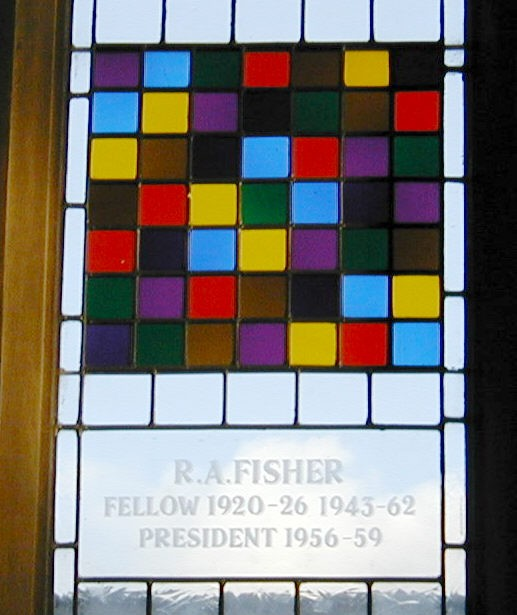
\includegraphics[scale = 0.18]{fisher.jpg}
            \end{figure}
        \end{column}%
    \end{columns}
    
\end{frame}


\begin{frame}{Пример: $E$-преобразование}
    Пусть $x_1, \ldots, x_k, \ell \in Q$.
    Определим~\footcite{markovski2017quasigroup} преобразование $E_{\ell}$:
    \[
        E_{\ell}(x_1 \ldots x_k) = y_1 \ldots y_k,
    \]
    \pause
    \[
        y_1 = \ell \circ x_1, \; y_{i+1} = y_i \circ x_{i+1}.
    \]
    \begin{figure}[h]
        \centering 
        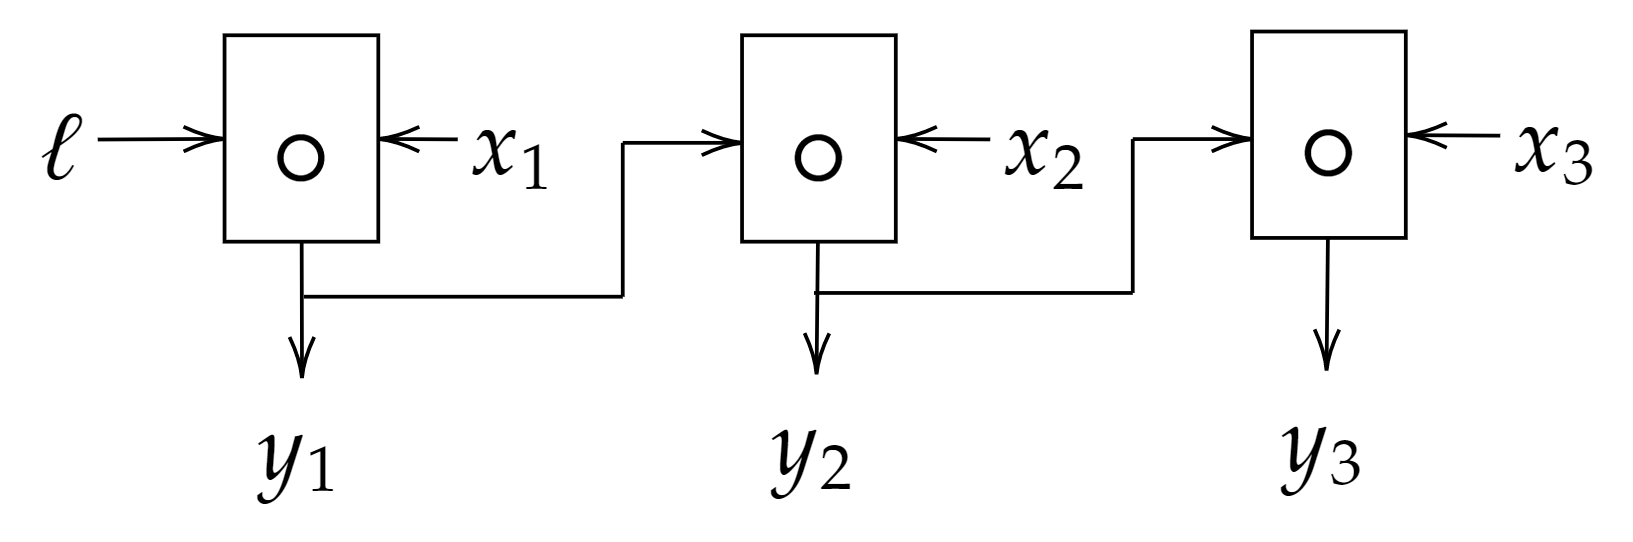
\includegraphics[width = 0.7\linewidth]{etransform.png}
    \end{figure}
\end{frame}


% \begin{frame}{Элементарные преобразования: $D$-преобразование}
%     \[
%         y_1 = \ell \circ x_1, \; y_{i+1} = y_i \circ x_{i+1}.
%     \]
%     \begin{coloritemize}
%         \item Даны $y_1, \ldots, y_k, \ell$, как обратить и получить $x_1, \ldots, x_k$?
%         \pause 
%         \item Нужно использовать операцию $\backslash$:
%         \[
%             a \circ b = c \Rightarrow b = a \backslash c.
%         \]
%         \pause 
%         \item Обращение:
%         \[
%             x_1 = \ell \backslash y_1, x_{i+1} = y_i \backslash y_{i+1}.
%         \]
%         \pause 
%         \item Обозначим полученное преобразование через $D_{\ell}$, тогда:
%         \[
%             D_{\ell} \left( E_{\ell}(x_1 \ldots x_k) \right) = E_{\ell} \left( D_{\ell} (x_1 \ldots x_k) \right) = (x_1 \ldots x_k).
%         \]
%     \end{coloritemize}
% \end{frame}


\begin{frame}{Пример: итерации $E$-преобразований}
    \begin{coloritemize}
        \item Пусть на $Q$ задано несколько структур квазигруппы: $\circ_1, \ldots, \circ_n$.
        \item Можем ввести кратное $E$-преобразование:
        \[
            E_{\ell_1, \ldots, \ell_n}(x) = E_{\ell_1} \left( \ldots \left( E_{\ell_n} (x) \right) \ldots \right), 
        \]
        \item Каждое $E_{\ell_i}$ использует свою операцию $\circ_i$.
        \pause
        \item Чтобы  \textquote{отменить}, нужно применить $D$, но в обратном порядке:
        \[
            D_{\ell_1, \ldots, \ell_n}(y) = D_{\ell_n} \left( \ldots \left( D_{\ell_1} (y) \right) \ldots \right).
        \]
    \end{coloritemize}
\end{frame}


\begin{frame}{Некоторые свойства $E$-преобразования}
    Работы~\footcite{markovski1999quasigroup, bakeva2011some, markovski2017quasigroup}.
    \begin{coloritemize}
        \item Для любых $\alpha = (a_1, \ldots, a_m)$ и $(c_1, \ldots, c_k)$ уравнение 
        \(
            E_{\alpha}(x_1 \ldots x_k) = c_1 \ldots c_k
        \)
        имеет единственное решение (в силу обратимости $E_{\alpha}$).
        \pause 
        \item Отображение $E_a \colon Q \to Q$ задает марковскую цепь: если $X_1 \ldots X_n$~--- случайные независимые величины, распределенные на $Q$, то распределение вероятностей знаков $Y_1 \ldots Y_n = E_a(X_1 \ldots X_n)$ задаются матрицей переходных вероятностей (распределение $Y_m$ зависит от распределения $Y_{m-1}$ и не зависит от $Y_{m-2}, \ldots, Y_1$).
        \pause 
        \item Распределение $Y_i$ сходится к равновероятному (для достаточно большого $n$, по свойству марковских цепей).
        \pause 
        \item Если применяем кратное $E$-преобразование с кратностью $\ell$, то распределение подстрок длины $\ell$ вида $Y_i Y_{i+1} \ldots Y_{i + \ell - 1}$ сходится к равновероятному (для достаточно большого $n$).
    \end{coloritemize}
\end{frame}


\begin{frame}{Механизмы}
    \begin{coloritemize}
        \item ГПСЧ на основе итерации $E$-преобразований~\footcite{dimitrova2004quasigroup, markovski2005unbiased}.
        \item Блочный шифр INRU~\footcite{inru}, $E$-преобразование используется в качестве нелинейного элемента.
        \item  \textquote{Односторонняя функция}~\footcite{gligoroski2008edon, gligoroski2009family, EdonR, EdonRprime} и основанные на ней хеш-функции:
        \begin{equation*}
            R(a_1 \ldots a_n) = E_{a_1} \left( \ldots E_{a_n}(a_1 \ldots a_n) \ldots \right).
        \end{equation*}
    \end{coloritemize}
\end{frame}


% \begin{frame}{Генераторы ПСЧ на основе $E$-преобразований}
%     \begin{coloritemize}
%         \item Раз все подстроки, получаемые с помощью $E$-преобразования, распределены  \textquote{хорошо}, то имеет смысл подумать о генераторе псевдослучайных чисел (ГПСЧ) на основе $E$-преобразований.
%         \item ГПСЧ: растягиваем короткий случайный вектор $seed$ на длинный псевдослучайный вектор-гамму.
%         \pause
%         \item Идея~\footcite{dimitrova2004quasigroup, markovski2005unbiased}: растягиваем короткий элемент $a \in Q$ с помощью итераций $E$-преобразования:
%         \[
%             E_{a} \left( \ldots E_{a} \left( E_{a} \left( a \ldots a \right) \right) \ldots \right).
%         \]
%         \begin{figure}[h]
%             \centering 
%             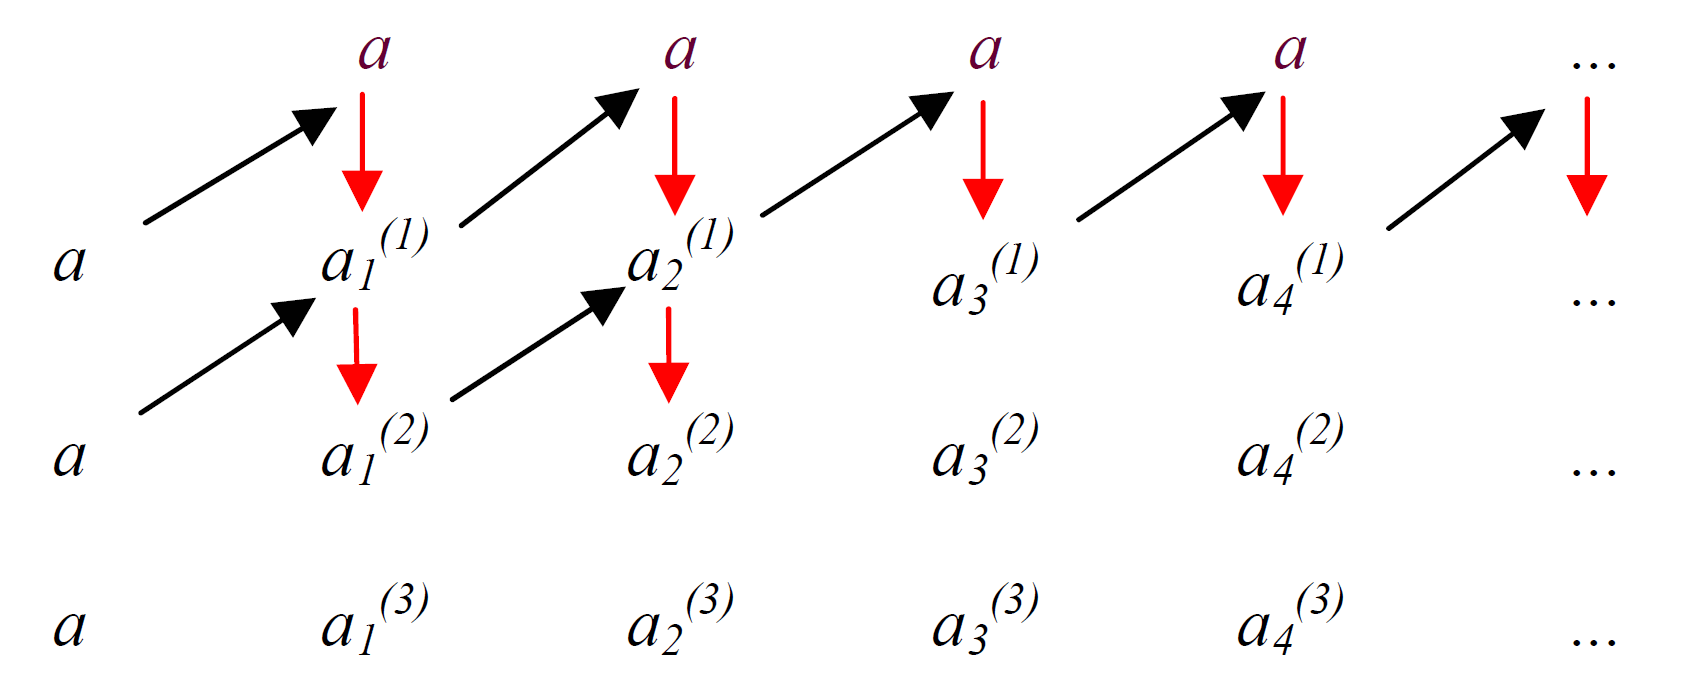
\includegraphics[width = 0.6\linewidth]{prng.png}
%         \end{figure}
%     \end{coloritemize}
% \end{frame}


% \begin{frame}{Некоторые свойства ГПСЧ на основе $E$-преобразований}
%     \begin{coloritemize}
%         \item Пусть $p_k$ есть период последовательности, полученной после $k$-кратного преобразования 
%         \(
%             E^k_{a} \left( a \ldots a \right).
%         \)
%         \item Тогда~\footcite{markovski2003quasigroup} $p_{p_{k-1}} > p_{k-1}$.
%         \item В частности~\footcite{markovski2005classification, markovski2005unbiased} период растет по крайней мере линейно с ростом $k$.
%         \pause
%         \item Можно ввести характеристику  \textquote{рост периода} (period growth), показывающую, насколько быстро растет период при итерациях преобразования $E_a$.
%         \item Как правило (статистические исследования): чем больше размер множества $Q$, тем больше шансов, что случайно выбранная квазигруппа $Q$ экспоненциально быстро увеличивает период последовательности~\footcite{markovski2005classification}.
%     \end{coloritemize}
% \end{frame}


% \begin{frame}{Пример: блочный шифр, основанный на $E$-преобразовании}
%     Работа~\footcite{inru}.
%     \begin{coloritemize}
%         \item INRU: блочный шифр, состоит из 16 раундов.
%         \pause 
%         \item Использует квазигруппу размера $16 \times 16$: полиномиально полная (т.е. лежит в классе  \textquote{хороших} с точки зрения теории сложности), не имеет собственных подквазигрупп, алгебраическая степень~--- 6.
%         \pause 
%         \item нелинейная часть: $E$-преобразования с ключом.
%     \end{coloritemize}
% \end{frame}


% \begin{frame}{INRU: структура шифра}
%     \begin{columns}[T] % gather columns
%         \begin{column}{.48\textwidth}
%             \begin{coloritemize}
%                 \item $E^{left}$, $E^{right}$~--- левое и правое $E$-преобразования;
%                 \item $\mathcal{L}$~--- некоторые линейные преобразования;
%                 \item $rk$~--- раундовый ключ.
%             \end{coloritemize}
%         \end{column}%
%         \hfill%
%         \begin{column}{.48\textwidth}
%             \begin{figure}[h]
%                 \centering 
%                 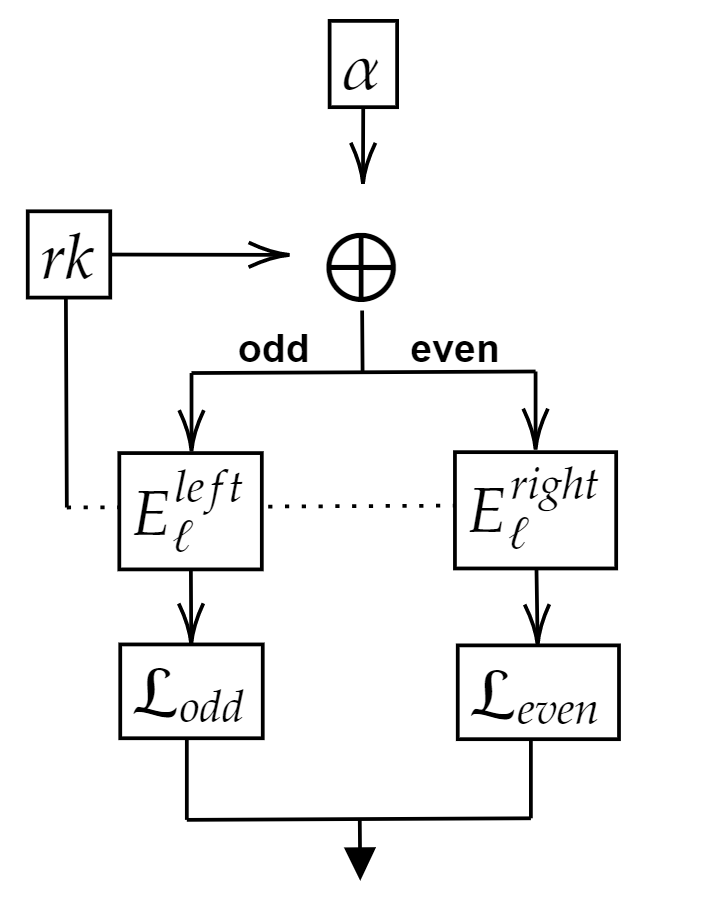
\includegraphics[width = 0.75\linewidth]{inru_round.png}
%             \end{figure} 
%         \end{column}%
%     \end{columns}
% \end{frame}


\begin{frame}{Другие предложения (кратко)}
    Основная идея: использовать в качестве нелинейного компонента примитива некоторое квазигрупповое преобразование.
    \begin{coloritemize}
        % \item  \textquote{Односторонняя функция}~\footcite{gligoroski2008edon, gligoroski2009family, EdonR, EdonRprime} и основанные на ней хеш-функции:
        % \begin{equation*}
        %     R(a_1 \ldots a_n) = E_{a_1} \left( \ldots E_{a_n}(a_1 \ldots a_n) \ldots \right).
        % \end{equation*}
        % \pause
        \item Низкоресурсная (легковесная/lightweight) хеш-функция GAGE и AEAD-алгоритм InGAGE (см.~\url{http://gageingage.org/}, также~\footcite{otte2019gage, gligoroski2019s}).
        \item Поточный шифр Edon80~\footcite{edon80}.
        \item Хэш-функция NaSHA~\footcite{mileva2009quasigroup}.
    \end{coloritemize}
\end{frame}


\begin{frame}{Другие предложения (кратко)-2}
    \begin{coloritemize}
        \item Асимметричные криптопримитивы~--- аналоги пост-квантовых схем multivariate cryptography~\footcite{preneel}.
        \pause
        \item Основная идея: подобрать такое нелинейное преобразование $\mathcal{P}$, что вычисление $\mathcal{P}$ и $\mathcal{P}^{-1}$ сделать  \textquote{легко}, а затем  \textquote{скрыть} структуру $\mathcal{P}$, взяв обратимые линейные преобразования $\mathcal{S}$ и $\mathcal{T}$ и рассмотрев композицию 
        \(
            \mathcal{F}(x) = \mathcal{S} \left( \mathcal{P} \left(\mathcal{T}(x) \right) \right).
        \)
        \pause 
        \item В работах~\footcite{gligoroski2008public, gligoroski2008multivariate, chen2010multivariate, gligoroski2011mqq} предлагалось рассматривать в качестве нелинейной компоненты $\mathcal{P}$ композицию $E$-преобразований.
        \pause 
        \item В работах~\footcite{mohamed2009algebraic, faugere2015polynomial} предлагаемая система и её модификации были успешно атакованы (решение задачи MinRank с помощью базисов Грёбнера).
    \end{coloritemize}
        
\end{frame}


\begin{frame}{Другие предложения (кратко)-3}
    \begin{coloritemize}
        \item Схемы~--- аналоги протокола Диффи-Хеллмана выработки общего ключа~\footcite{katyshev14, katyshev18}, гомоморфное шифрование~\footcite{gribov2010construction, gribov15, markov20}: используются ППС/ПЛС-группоиды, луповые кольца над медиальными квазигруппами (изотопы абелевых групп с коммутирующими автоморфизмами).
        \pause
        \item Приложения в теории кодирования~\footcite{nechaev98, nechaev04, couselo2004loop, markov12, markov2020nonassociative}...
        \pause 
        \item и многое другое~\footcite{glukhov, artamonov18, shcherbacov2017elements}.
    \end{coloritemize}
\end{frame}


\begin{frame}{Как задать квазигруппу?}
    \begin{coloritemize}
        \item В общем случае квазигруппа над множеством $Q$ задается таблицей умножения размера $\lvert Q \rvert \times \lvert Q \rvert$; это много.
        \pause 
        \item Случайная генерация (поиск + отсев) квазигрупп из некоторого узкого класса~\footcite{gligoroski2008public, chen2010multivariate}.
        \pause 
        \item Итеративное построение из более \textquote{маленьких} (конструкции наподобие прямых произведений)~\footcite{gribovphd, EdonRprime}.
        \pause 
        \item Изотопы некоторых \textquote{хорошо изученных} групп (например, изотоп группы точек эллиптической кривой~\footcite{DH16}, модульное вычитание~\footcite{snavsel2009hash}).
        \pause 
        \item Функциональное задание квазигруппы: поговорим о нём подробнее.
    \end{coloritemize}
\end{frame}


\begin{frame}{Функциональное задание квазигруппы}
    \begin{coloritemize}
        \item Можно перейти от табличного задания операции к функциональному~\footcite{nosov08}: 
        \[
            x \circ y = z \leftrightarrow z_i = f_i(x_1, \ldots, x_n, y_1, \ldots, y_n). 
        \]
        \pause 
        \item Рассмотрим для простоты случай $Q = \{0, 1\}^n$: хотим задать структуру квазигруппы на $Q$ с помощью семейства булевых функций.
        \pause 
        \item Какие условия надо наложить на функции $f_i$, чтобы операция $x \circ y$ задавала структуру квазигруппы на $Q$?
    \end{coloritemize}
\end{frame}


\section{Правильные семейства функций}


\begin{frame}{Правильные семейства булевых функций}
    \begin{myexample}{Правильное семейство}
        Семейство булевых функций $f_i \colon \EE_2^n \to \EE_2^n$ называется правильным, если для любых двух наборов $x \ne y$ найдется такая координата $i$, что $x_i \ne y_i$, но $f_i(x) = f_i(y)$ (см.~\footcite{nosov98, nosov99}).
    \end{myexample}
    \pause 

    Правильные семейства можно задавать не только над $\EE_2^n$, но над логикой любой значности $k$~\footcite{nosov06}, над произвольными группами~\footcite{nosov06abel}; над прямыми произведениями других квазигрупп~\footcite{galatenko2020latin} и даже $d$-квазигрупп~\footcite{plaksina14}.
\end{frame}


\begin{frame}{Правильные семейства и квазигруппы}
    Семейство булевых функций $F = (f_1, \ldots, f_n)$ является правильным тогда и только тогда, когда отображение вида 
    \[
        (x, y) \to z = x \oplus y \oplus F(\pi_1(x_1, y_1), \ldots, \pi_n(x_n, y_n))
    \]
    задает квазигрупповую операцию \textbf{при любом выборе} внутренних функций $\pi_1, \ldots, \pi_n$.

    \pause 
    \begin{mypropos}{Существенная (не)зависимость}
        Из определения правильности следует, что $f_i$ не зависит существенно от $x_i$.
    \end{mypropos}
\end{frame}


\begin{frame}%{Примеры правильных семейств}
    \begin{mypropos}{Константные семейства}
        $f_i \equiv const_i$ является правильным.
    \end{mypropos}
    \pause 
    \begin{mypropos}{Треугольные семейства}
        \[
            \begin{bmatrix}
                f_1 \\
                f_2 \\
                f_3 \\
                \vdots \\
                f_n 
            \end{bmatrix}
            =
            \begin{bmatrix}
                const \\
                f_{2}(x_{1}) \\
                f_{3}(x_{1}, x_{2}) \\
                \vdots \\
                f_{n}(x_{1}, \ldots, x_{n-1})
            \end{bmatrix}
        \]
        является правильным~\footcite{nosov06abel}.
    \end{mypropos}
\end{frame}


\begin{frame}%{Примеры правильных семейств-2}
    \begin{myexample}{Ортогональные функции}
        Две функции $f, g \colon \EE_k^n \to \EE_k$ будем называть \textbf{ортогональными}, если для любого $x \in \EE_k^n$ выполняется хотя бы одно из двух равенств: $f(x) = 0$ или $g(x) = 0$. 
    \end{myexample}
    \pause
    \begin{mypropos}{Семейство ортогональных функций}
        Пусть $F = (f_1, \ldots, f_n)$~--- семейство попарно ортогональных функций, и $f_i$ не зависит существенно от $x_i$.
        Тогда $F$ является правильным~\footcite{nosov08}. 
        \begin{gather*}
            \label{OrthogExample}
            f_1 =\bar{x}_2 x_3 \cdots x_{n-1} x_n,\\
            f_2 =\bar{x}_3 x_4 \cdots x_{n} x_1,\\
            \vdots \\
            f_n =\bar{x}_1 x_2 \cdots x_{n-2} x_{n-1}
        \end{gather*}
    \end{mypropos}
\end{frame}


\begin{frame}%{Примеры правильных семейств-3}
    \begin{mytheorem}{Класс квадратичных семейств}
        Семейство $F$ вида~\ref{quadratic} является правильным для любого $n \ge 1$:
        \begin{equation}
            \label{quadratic}
            \begin{bmatrix}
            0 \\
            x_1 \\
            x_1 \oplus x_2 \\
            \vdots \\
            x_1 \oplus x_2 \oplus \ldots \oplus x_{n-1}
            \end{bmatrix}
            \bigoplus
            \begin{bmatrix}
            \bigoplus_{i < j, \; i, j \ne 1}^n \; x_i x_j \\
            \bigoplus_{i < j, \; i, j \ne 2}^n \; x_i x_j \\
            \bigoplus_{i < j, \; i, j \ne 3}^n \; x_i x_j \\
            \vdots \\
            \bigoplus_{i < j, \; i, j \ne n}^n \; x_i x_j \\
            \end{bmatrix}.
        \end{equation}
    \end{mytheorem}
    \footcitetext{dm21}
\end{frame}


\begin{frame}{Преобразования, сохраняющие правильность}
    \begin{mypropos}{Преобразование сдвига}
        \label{thm:shift}
        Для любого $\alpha = (a_1, \ldots, a_n) \in Q^n$ определим преобразование сдвига~\footcite{nosov08}:
        \begin{gather*}
            x \in Q^n \to L_{\alpha}(x) = (a_1 \circ x_1, \ldots, a_n \circ x_n), \\
            x \in Q^n \to R_{\alpha}(x) = (x_1 \circ a_1, \ldots, x_n \circ a_n).
        \end{gather*}
        \pause
        Если $F \colon Q^n \to Q^n$ правильное, то $T_{\alpha}(F(T_{\beta}(x)))$ также правильное, где $T \in \{L, R\}$, $\alpha, \beta \in Q^n$.
    \end{mypropos}
\end{frame}


\begin{frame}{Преобразования, сохраняющие правильность-2}
    \begin{mypropos}{Преобразование перекодировки}
        \label{thm:reencoding}
        Для любого набора $\Psi = (\psi_1, \ldots, \psi_n) \in Func(Q)^n$ определим преобразование перекодировки:
        \[
            x \in Q^n \to \Psi(x) = (\psi_1(x_1), \ldots, \psi_n(x_n)).
        \]
        Пусть $\Phi \in Func(Q)^n$, $\Psi \in Perm(Q)^n$.
        Если $F(x) = (f_1(x), \ldots, f_n(x))$ правильное, то $\Phi(F(\Psi(x)))$ также правильное.
    \end{mypropos}
    \pause
    Если $\Phi, \Psi \in Perm(Q)^n$, то подобные преобразования будем называть преобразованиями перекодировки.
    \pause
    \begin{mypropos}{Замечание}
        Сдвиги являются частными случаями преобразования перекодировки.
    \end{mypropos}
\end{frame}


\begin{frame}{Преобразования, сохраняющие правильность-3}
    \begin{mypropos}{Согласованная перенумерация}
        Пусть $\sigma \in Perm(n)$, определим преобразование согласованной перенумерации:
        \begin{gather*}
            F \to \sigma(F), \\
            f_i(x_1, \ldots, x_n) \to 
            f_{\sigma(i)}(x_{\sigma(1)}, \ldots, x_{\sigma(n)}).
        \end{gather*}
        \pause
        Если $F(x)$~--- правильное, то $\sigma(F)$ также правильное~\footcite{nosov08}.
    \end{mypropos}
\end{frame}


\begin{frame}{Преобразования, сохраняющие правильность-4}
    \begin{mypropos}{Проекция}
        Подставим значение $a \in Q$ вместо переменной $x_i$ и исключим функцию $f_i$, $1 \le i \le n$.
        \[
            F'(x_1,\ldots,x_{i-1}, x_{i+1}, \ldots, x_n) = \proj^i_a(F) =
            \begin{bmatrix}
              f_1(x_1,\ldots,x_{i-1}, a, x_{i+1}, \ldots, x_n) \\
              \vdots \\
              f_{i-1}(x_1,\ldots,x_{i-1}, a, x_{i+1}, \ldots, x_n) \\
              f_{i+1}(x_1,\ldots,x_{i-1}, a, x_{i+1}, \ldots, x_n) \\
              \vdots \\
              f_{n}(x_1,\ldots,x_{i-1}, a, x_{i+1}, \ldots, x_n) \\
            \end{bmatrix}.
        \]
        Полученное семейство является правильным.
    \end{mypropos}
\end{frame}


\begin{frame}{Общий вид биекций, сохраняющих правильность}
    \begin{coloritemize}
        \item Пусть $\Phi$, $\Psi$~--- биекции на $Q^n$: $\Phi, \Psi \in Perm(Q^n)$.
        Рассмотрим стабилизатор множества всех правильных семейств, заданных на $Q^n$:
        \[
            \{(\Phi, \Psi) \in Perm(Q^n) \mid \Phi(F(\Psi(x))) \text{ правильно для любого правильного } F \colon Q^n \to Q^n \}.  
        \]
        \pause
        \item Тогда $\Phi$ и $\Psi$ должны быть изометриями $Q^n$ (в метрике Хэмминга).
        \pause
        \item Изометрии $\EE_k^n$, $\lvert Q \rvert = k$~--- это перенумерации и перекодировки.
        \pause
        \item Оба этих класса преобразований сохраняют правильность (перенумерации должны быть согласованы).
    \end{coloritemize}   
\end{frame}


\begin{frame}{Общий вид биекций, сохраняющих правильность}
    \begin{mytheorem}{Стабилизатор правильных семейств}
        Пусть семейства $\gf(\xx)$ вида $\gf(\xx) = \Phi(\ff(\Psi(\xx)))$ являются правильным для всех правильных семейств $\ff$, заданных на $\EE_k^n$, $\Phi$ и $\Psi$~--- биекции множества $\EE_k^n$.
        Тогда $\Phi$ и $\Psi$ имеют вид 
        \[
            \Phi = \sigma \circ A, \Psi = \sigma \circ B, 
        \]
        где использованы следующие обозначения:
        \begin{description}
            \item[$\sigma \in \SSS_n$:] перенумерация координат вектора,
            \item[$A, B \in \left( \SSS_{\EE_k} \right)^n$:] перекодировки вектора. 
        \end{description}
    \end{mytheorem}
\end{frame}


\begin{frame}{Открытые вопросы-1}
    \begin{coloritemize}
        \item Построение достаточно широких классов правильных семейств с \textquote{хорошими} свойствами, в том числе и для логик большей значности $k > 2$?
        \pause 
        \item Есть отношение эквивалентности на множестве правильных семейств, как быстро строить представителей?
        \pause 
        \item Можно ли поставить классам эквивалентности во взаимно-однозначное соответствие какие-то геометрические объекты, группы симметрий которых соответствуют согласованным перенумерациям и перекодировкам (для логик значности $k > 2$)?
    \end{coloritemize}
\end{frame}


\section{Эквивалентные определения правильности}


\begin{frame}{Одностоковые ориентации ($\uso$)}
    \begin{myexample}{Булев куб  $\BB_n$}
        \begin{coloritemize}
            \item вершины: $V = \{ \alpha \in \EE_2^n \}$;
            \item ребра: $\{\alpha, \beta \} \in E \Leftrightarrow \rho(\alpha, \beta) = 1$ (расстояние Хэмминга).
        \end{coloritemize}
    \end{myexample}
    \pause 
    \begin{myexample}{Ориентация с единственным стоком $\uso$}
        \textbf{Ориентация с единственным стоком}~\footcite{szabo2001} (unique sink orientation, $\uso$) куба $\BB_n$~--- ориентированный граф, построенный по $\BB_n$ со следующим характеристическим свойством: в каждом подкубе $\BB_n$ существует единственный сток.
    \end{myexample}
\end{frame}  

  
\begin{frame}{$\uso$: один пример}
    \begin{figure}
          \centering
          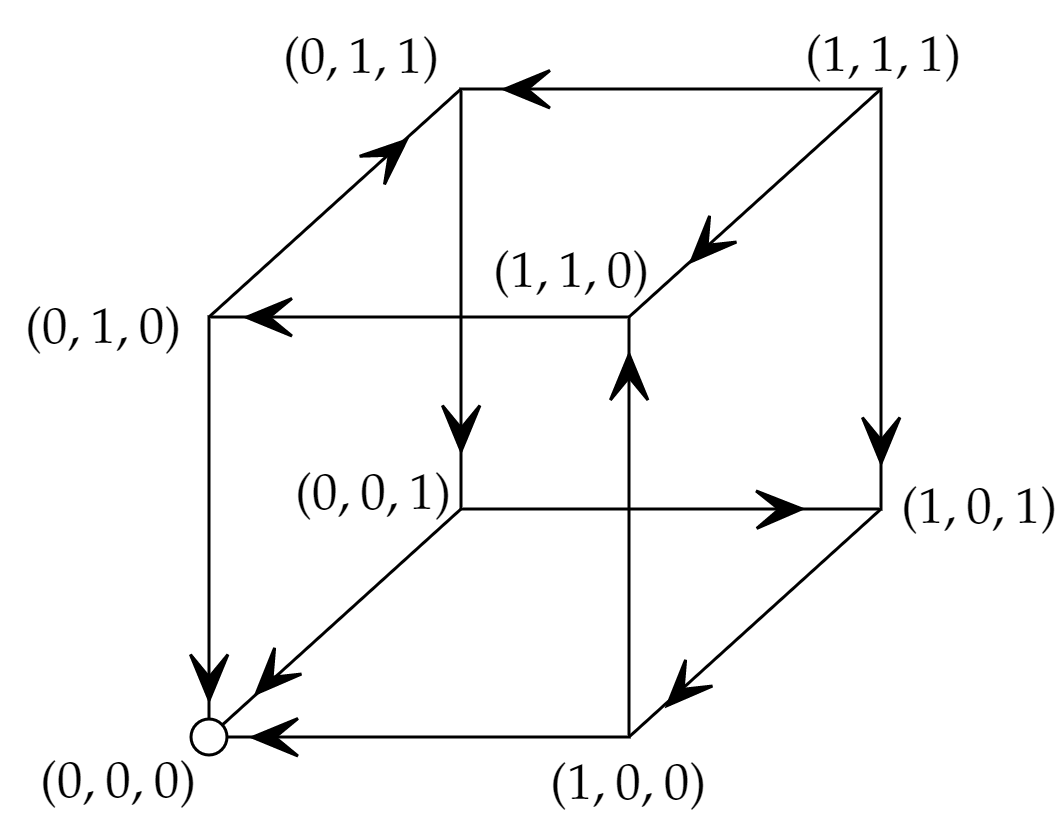
\includegraphics[width=0.45\linewidth]{USO.png}
          \caption{Одностоковая ориентация трехмерного булева куба $\BB_3$}
    \end{figure}
\end{frame}


\begin{frame}%{Граф семейства $\Gamma(F)$}
    Пусть $F$~--- семейство булевых функций.
    \begin{myexample}{Граф семейства $\Gamma(F)$}
        \begin{coloritemize}
            \item Вершины: $V = \{ \alpha \in \EE_2^n \}$.
            \item Пусть $\alpha \ne \beta$, $\rho(\alpha, \beta) = 1$, $\alpha_i \ne \beta_i$, добавим ориентированное ребро $(\beta, \alpha) \in E$ тогда и только тогда, когда $f_i(\alpha) = \alpha_i$.
        \end{coloritemize}
    \end{myexample}
    \pause
    \begin{figure}
        \centering
        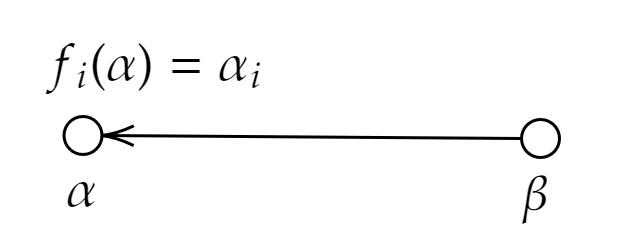
\includegraphics[width=0.45\linewidth]{edge.png}
    \end{figure}
\end{frame}


\begin{frame}{Неподвижные точки графа $\Gamma(F)$}
    \begin{figure}
        \centering
        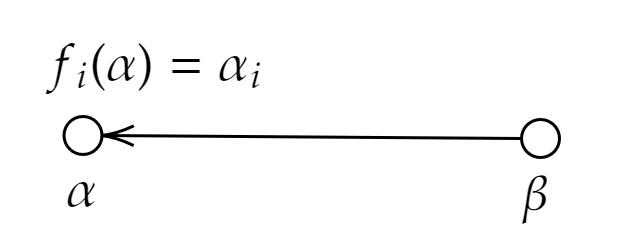
\includegraphics[width=0.45\linewidth]{edge.png}
    \end{figure}
    \begin{coloritemize}
        \item Чему в терминах графа $\Gamma(F)$ соответствует неподвижная точка $\alpha$ отображения $x \to F(x)$?
        \pause
        \item $f_i(\alpha) = \alpha_i$ для всех $1 \le i \le n$.
        \pause 
        \item Следовательно, $\alpha$~--- сток в $\Gamma(F)$.
        \pause 
        \item Ориентации подкубов в $\Gamma(F)$ задаются проекциями $F'$ семейства $F$.
    \end{coloritemize}
\end{frame}


\begin{frame}{$\uso$ и правильность: два описания одного объекта}  
    \begin{mytheorem}{Взаимно-однозначное соответствие}
        Граф $\Gamma(F)$ семейства булевых функций $F$ является одностоковой ориентацией тогда и только тогда, когда $F$~--- правильное семейство~\footcite{intsys20, pdm20}.
    \end{mytheorem}
    \pause
    \begin{coloritemize}
        \item Существует взаимно-однозначное соответствие между \textquote{алгебраическим} и \textquote{геометрическим}описаниями.
        \item Это позволяет переводить результаты с одного \textquote{языка}на другой.
        \item Некоторые примеры переноса: вероятностный алгоритм порождения правильных семейств с помощью процедуры MCMC~\footcite{USOphd, galatenko21}, оценка на число булевых правильных семейств~\footcite{dm21}, новые классы правильных семейств.
    \end{coloritemize}    
\end{frame}


\begin{frame}{Рекурсивная треугольность}
    \begin{block}{Рекурсивная ориентация}
        Рекурсивно одностоковая ориентация булева $n$-мерного куба $\EE_n$ задается следующим характеристическим свойством: найдется такое направление $i$, вдоль которой все ребра ориентированы в одном направлении, и ориентация на каждом из подкубов $x_i = 0$ и $x_i = 1$ размерности $(n-1)$ также является рекурсивно одностоковой (recursively combed cube orientation~\footcite{gao2020new}).
    \end{block}
    \pause 
    \begin{mytheorem}{Рекурсивно треугольное семейство}
        Семейство $F \colon \EE_k^n \to \EE_k^n$ со свойством: существует $i$, такое что $f_i \equiv const_i$, и $\proj_a^i(F)$ рекурсивно треугольны для всех $a \in \EE_k$.
    \end{mytheorem}
\end{frame}


\begin{frame}{Рекурсивная треугольность}
    \begin{mytheorem}{Замечание}
        Рекурсивно треугольные семейства более общее понятие, чем треугольные: треугольные семейства являются такими рекурсивно треугольными, что каждая из проекций $\proj^a_i(F)$ постоянна вдоль одного и того же направления~$j$.
    \end{mytheorem}
    \pause
    \begin{mytheorem}{Теорема}
        Рекурсивно треугольные семейства являются правильными.
    \end{mytheorem}
\end{frame}


\begin{frame}%{Почти все булевы правильные семейства не треугольны}
    Пусть $T(n)$ ($\Delta(n)$)~--- число \textbf{булевых} правильных (треугольных) семейств размера~$n$.
    \pause
    \begin{mypropos}{Оценка на число булевых правильных семейств}
        \[
            n^{A \cdot 2^n} \le T(n) \le n^{B \cdot 2^n},
        \]
        где $A$, $B$~--- некоторые положительные константы~\footcite{numberUSO}.
    \end{mypropos}
    \pause 
    \begin{mytheorem}{Булевых треугольных семейств экспоненциально мало}
    \label{ThTri}
        \[
            \frac{\Delta(n)}{T(n)} = o \Big(\frac{1}{n^{D \cdot 2^n}} \Big) \text{ при } n \to \infty,
        \]
        для некоторого $D > 0$~\footcite{dm21}.
        Таким образом, почти все булевы правильные семейства не являются треугольными.
    \end{mytheorem}
\end{frame}


\begin{frame}{Рекуррентное соотношение}
    \begin{mytheorem}{Число рекурсивно треугольных семейств}
        Пусть $\Delta^{\rec}(n)$~--- число рекурсивно треугольных семейств размера~$n$ над $k$-значной логикой.
        Тогда выполняется равенство:
        \[
            \Delta^{\rec}(n) = \sum_{j=1}^{n} (-1)^{j+1} \cdot k^j \cdot {n \choose j} \Delta^{\rec}(n-j)^{k^j}.
        \]
    \end{mytheorem}
    \pause 
    \begin{mytheorem}{Замечание}
        Доля булевых рекурсивно треугольных семейств размера $n$ в классе всех булевых правильных семейств размера $n$ стремится к 0 при $n \to \infty$. 
    \end{mytheorem}
\end{frame}


\begin{frame}{Сложность распознавания правильности}
    \begin{coloritemize}
        \item В общем случае проверка правильности является сложной задачей: если семейство задано в форме КНФ, то задача проверки правильности coNP-полна~\footcite{nosov98}.
        \pause 
        \item В определенных случаях задача проверки правильности может быть упрощена, в частности, за счет вида графа существенной зависимости~\footcite{rykov14}.
        \pause 
        \item Алгоритм проверки правильности булева семейства требует порядка $\Theta(4^n)$ операций вычисления правильного семейства на двоичном наборе $x$ (проверка по определению правильности).
        \pause 
        \item Предложена адаптация алгоритма~\footcite{bosshard2017pseudo} со сложностью $\Theta(3^n)$, проверяющего, что ориентация $\Gamma(F)$, задаваемая семейством $F$, является одностоковой.
        \pause 
        \item Алгоритм опирается на еще одно характеристическое свойство правильных семейств: булево семейство правильно тогда и только тогда, когда каждая его проекция не является самодвойственным отображением.
    \end{coloritemize}
\end{frame}


\begin{frame}{Неподвижные точки правильного семейства}
    \begin{mytheorem}{Булев случай}
        Булево семейство $F$ является правильным тогда и только тогда, когда семейство $F$ и каждая из его проекций имеет единственную неподвижную точку.
    \end{mytheorem}
    \pause 
    \begin{mypropos}{Общий случай}
        Семейство $F \colon \EE_k^n \to \EE_k^n$ является правильным тогда и только тогда, когда для любой перекодировки $F$ все её проекции имеют единственную неподвижную точку.
    \end{mypropos}
    \pause 
    В булевом случае свойство единственности неподвижной точки дает ещё одно характеристическое свойство правильных семейств, которое изучалось в контексте математической биологии (в частности, при изучении экспрессии генов~\footcite{thomas1991regulatory, richard2015fixed, ruet2015asynchronous, ruet2016local}).    
\end{frame}


\begin{frame}%{$\hupf$-сети}
    \begin{myexample}{Булевы сети с наследственно единственной неподвижной точкой}
        $\hupf$-сеть (сеть с наследственно единственной неподвижной точкой, hereditarily unique fixed point network)~--- булево семейство $F$ со следующим свойством: $F$ и все его проекции имеют единственную неподвижную точку (как отображения $\EE_2^n \to \EE_2^n$).
    \end{myexample}
    \pause 
    \begin{mytheorem}{Правильные семейства $\leftrightarrow$ $\hupf$-сети}
        Булево семейство $F$ является правильным $\Leftrightarrow$ $F$ задает $\hupf$-сеть. 
    \end{mytheorem}
    \pause
    Соответствие между булевыми правильными семействами и $\hupf$-сетями позволяет перенести (и обобщить) часть результатов, полученных в контексте изучения динамики таких сетей, на правильные семейства.
\end{frame}


\begin{frame}%{Глобальный граф взаимодействий}
    Пусть $F$~--- семейство размера $n$.
    \begin{myexample}{Глобальный граф взаимодействий $G(F)$}
        \begin{coloritemize}
        \item Вершины: $V = \{1, \ldots, n\}$.
        \item Ребра: $i \to j$ тогда и только тогда, когда $f_j$ существенно зависит от $x_i$.
        \item Эквивалентно: \textquote{дискретная} частная производная $f_j$ по $x_i$ не равна тождественно нулю.
        \end{coloritemize}
    \end{myexample}
    \pause
    \begin{mypropos}{Ациклические глобальные графы}
        Если $G(F)$~--- ациклический, то $F$~--- $\mathsf{HUPF}$-сеть~\footcite{robert1980iterations}.
    \end{mypropos}
    \pause 
    Эквивалентно: если $F$~--- булево треугольное семейство, то $F$ правильно.
\end{frame}


\begin{frame}%{Локальный граф взаимодействий}
    Пусть $F$~--- семейство размера $n$.
    \begin{myexample}{{Локальный граф взаимодействий $G(F, \alpha)$}}
        \begin{coloritemize}
        \item Вершины: $V = \{1, \ldots, n\}$.
        \item Ребра: $i \to j$ тогда и только тогда, когда $f_j$ существенно зависит от $x_i$  \textquote{локально} в точке $a$:
        \[
            f_j(\alpha_1, \ldots, \alpha_i, \ldots, \alpha_n) \ne f_j(\alpha_1, \ldots, \alpha_i \oplus 1, \ldots, \alpha_n).
        \]
        \end{coloritemize}
    \end{myexample}
    \pause 
    \begin{mypropos}{Ациклические локальные графы}
        Пусть $G(F, \alpha)$~--- ациклический для каждой точки $\alpha \in \EE_2^n$, тогда $F$~--- $\hupf$-сеть~\footcite{shih2005combinatorial}.
    \end{mypropos}
\end{frame}


\begin{frame}{Локальный граф взаимодействий-2}
    \begin{myexample}{Локально треугольные семейства}
        $F \colon \EE_k^n \to \EE_k^n $ локально треугольно, если $G(F, \alpha)$ ацикличен для каждой точки $\alpha \in \EE_k^n$, где локальная зависимость $f$ от $x_i$ в точке $\alpha$ определяется неравенством:
        \[
            \exists b \colon f(\alpha_1, \ldots, \alpha_i, \ldots, \alpha_n) \ne f(\alpha_1, \ldots, b, \ldots, \alpha_n).
        \]
    \end{myexample}
    \pause 
    \begin{mytheorem}{Теорема}
        Локально треугольные семейства являются правильными (в логиках любой значности).
    \end{mytheorem}
    \pause
    \begin{mytheorem}{Теорема}
        Всякое рекурсивно треугольное семейство является локально треугольным.
    \end{mytheorem}
\end{frame}


\begin{frame}{Локальный граф взаимодействий-3}
    Пусть $F$~--- семейство размера $n$.
    \begin{mypropos}{Теорема}
        Если для любого $t$, $1 \le t \le n$ существует не более $2^t - 1$ наборов $\alpha$, таких что $G(F, \alpha)$ имеет цикл длины не более чем $t$, то $F$ является $\mathsf{HUPF}$-сетью.
    \end{mypropos}
    \pause
    \begin{coloritemize}
        \item Непонятно, является ли это условие критерием.
        \item Интуитивная интерпретация /  \textquote{перевод} на язык правильных семейств общего вида пока что отсутствуют.
    \end{coloritemize}
\end{frame}


% \begin{frame}{Характеризация через несамодвойственные проекции}
%     \begin{block}{Самодвойственное семейство}
%         Отображение $F \colon \EE_2^n \to \EE_2^k$ самодвойственно, если для любого набора $x \in \EE_2^n$ выполняется свойство $F(\overline{x}) = \overline{F(x)}$.
%     \end{block}
%     \pause 
%     \begin{mytheorem}{О несамодвойственности проекций} 
%         Семейство $F$ булевых функций правильно тогда и только тогда, когда каждая из его проекций 
%         \[
%             \proj^{a_1, \ldots, a_k}_{i_1, \ldots, i_k}(F)
%         \] 
%         \textbf{не является} самодвойственным булевым отображением.
%     \end{mytheorem}
% \end{frame}


\begin{frame}{Кликовое представление правильных семейств}
    \begin{coloritemize}
        \item Правильные семейства находятся во взаимно-однозначном соответствии с кликами некоторым образом построенного графа (\textquote{обобщенный граф Келлера}).
        \item Для $k=2$ перенос из теории $\mathsf{USO}$-ориентаций~\footcite{borzechowski2022universal}, для $k > 2$~--- авторское обобщение.
        \item Обобщенный граф Келлера $G(k, n)$: $V = \EE_{k^2}^n$, 
        \[
            \{v, w\} \in E \leftrightarrow \exists i, \, 1 \le i \le n \colon v_i \equiv w_i \text{ mod } \; k, \; v_i \ne w_i.
        \]
        \item Графы примечательны тем, что в случае $k = 2$ некоторым образом кодируют неэквивалентные замощения пространства гиперкубами~\footcite{sikiric2007cube, mathew2013enumerating}.
    \end{coloritemize}
    \begin{mytheorem}{Соответствие между семействами и кликами}
        Каждой клике на $k^n$ вершинах в графе $G(k, n)$ можно поставить в биективное соответствие некоторое правильное семейство $\ff_n$ размера $n$ на $\EE_k^n$.
    \end{mytheorem}
\end{frame}


\begin{frame}{Ещё одна альтернативная характеризация}
    Существует ещё несколько альтернативных характеризаций правильных семейств.
    \begin{coloritemize}
        \item (Не)ортогональность аффинных пространств, построенных по правильным семействам.
    \end{coloritemize}
\end{frame}


\begin{frame}{Открытые вопросы-2}
    \begin{coloritemize}
        \item Больше эквивалентных определений правильных семейств для логик значности $k > 2$.
        \pause 
        \item В чем \textquote{глубинная} причина того, что некоторые эквивалентности  \textquote{работают} только в случае $k = 2$ и  \textquote{ломаются} при переходе к $k > 2$?
        \pause 
        \item Дальнейший перенос и обобщение результатов, полученных в рамках исследований $\hupf$-сетей и одностоковых ориентаций.
    \end{coloritemize}
\end{frame}


\section{Свойства правильных семейств}


\begin{frame}{Мощность образа правильного семейства}
    Пусть $F = (f_1, \ldots, f_n)$~--- правильное, тогда отображение вида 
    \[
        (x, y) \to z = x \oplus y \oplus f(\pi_1(x_1, y_1), \ldots, \pi_n(x_n, y_n))
    \]
    задает квазигрупповую операцию \textbf{при любом выборе} $\pi_1, \ldots, \pi_n$.
    \pause 
    \begin{coloritemize}
        \item Сколько может получиться \textbf{различных} квазигрупп при разных $\pi_1, \ldots, \pi_n$?
        \pause 
        \item Плохой пример: если все $f_i \equiv const_i$, то смена $\pi_i$ ничего не даст.
        \pause
        \item Оказывается, что количество порождаемых квазигрупп одним правильным семейством $F$ зависит от мощности образа этого семейства~\footcite{galatenko23}.
    \end{coloritemize}
    \begin{myexample}{Связь мощности образа и количества порождаемых квазигрупп}
        Пусть $F \colon \EE_k^n \to \EE_k^n$~--- правильное семейство, $M$~--- мощность образа отображения $x \to F(x)$.
        Тогда число различных квазигрупп, порождаемых указанной конструкцией, не менее чем $M^{k^2}$.
    \end{myexample}
\end{frame}


\begin{frame}%{Мощности образов некоторых конкретных правильных семейств}

    \begin{mypropos}{Ограниченность мощности образа}
        Число значений, принимаемых правильным семейством порядка~$n$ в $k$-значной логике, не превосходит~$k^{n-1}$ (см.~\footcite{galatenko23}).
    \end{mypropos}

    \begin{mytheorem}{Мощность образа квадратичного семейства}
        Семейство 
        \begin{equation}
            \begin{bmatrix}
            0 \\
            x_1 \\
            \vdots \\
            x_1 \oplus x_2 \oplus \ldots \oplus x_{n-1}
            \end{bmatrix}
            \bigoplus
            \begin{bmatrix}
            \bigoplus_{i < j, \; i, j \ne 1}^n \; x_i x_j \\
            \bigoplus_{i < j, \; i, j \ne 2}^n \; x_i x_j \\
            \vdots \\
            \bigoplus_{i < j, \; i, j \ne n}^n \; x_i x_j \\
            \end{bmatrix}
        \end{equation}
        имеет максимальную мощность образа~$2^{n-1}$.
    \end{mytheorem}
\end{frame}


\begin{frame}%{Мощности образов некоторых конкретных правильных семейств-2}
    \begin{equation}
        \label{stronglyquadratic}
        \begin{bmatrix}
            f_1(x_1, \ldots, x_n) \\
            f_2(x_1, \ldots, x_n) \\
            \vdots \\
            f_n(x_1, \ldots, x_n) \\
        \end{bmatrix}
        =
        \begin{bmatrix}
            \overline{x}_2 \cdot x_3 \\
            \overline{x}_3 \cdot x_4 \\
            \vdots \\
            \overline{x}_1 \cdot x_2 \\
        \end{bmatrix}.
    \end{equation}
    \pause
    \begin{mypropos}{Правильность семейства}
        Семейство~(\ref{stronglyquadratic}) является правильным.
    \end{mypropos}
    \pause
    \begin{mytheorem}{Мощность образа семейства}
        Мощность образа семейства~(\ref{stronglyquadratic}) равна $\lucas_n$ ($n$-е число Люка):
        \[
            \lucas_n = \lucas_{n-1} + \lucas_{n-2}, \quad \lucas_0 = 2, \lucas_1 = 1.
        \]
    \end{mytheorem}
\end{frame}


\begin{frame}{Подстановки, порождаемые правильными семействами}
    Пусть $F \colon Q^n \to Q^n$~--- правильное, $(Q, \circ)$~--- квазигруппа.
    Тогда отображение
    \[ 
        \sigma_F(x) \colon x \to x \circ F(x),
        \quad
        \begin{bmatrix}
            x_1 \\
            \vdots \\
            x_n
        \end{bmatrix} 
        \to 
        \begin{bmatrix}
            x_1 \circ f_1(x_1, \ldots, x_n) \\
            \vdots \\
            x_n \circ f_n(x_1, \ldots, x_n)
        \end{bmatrix}
    \]
    является подстановкой: $\sigma_F \in Perm(Q^n)$.
\end{frame}


\begin{frame}%{Обращение подстановок, порожденных правильными семействами}
    Пусть $F \colon Q^n \to Q^n$~--- правильное.
    Рассмотрим $\sigma^{-1}_F \in Perm(Q^n)$.
    \begin{mytheorem}{Обратимость \textquote{правильных подстановок}}
        Если $(Q, +)$~--- группа (т.е., операция $+$ ассоциативна), то семейство $G \colon Q^n \to Q^n$, определенное равенством
        \[
            G(x) = (-x) + \sigma_F^{-1}(x)
        \]
        также является правильным.
    \end{mytheorem}
    \pause
    Т.е., если $F$~--- правильное, то существует правильное семейство $G$ со свойством
    \[
        \sigma^{-1}_F(x) = \sigma_G(x).
    \]
    \pause
    Таким образом, множество \textquote{правильных подстановок} замкнуто относительно взятия обратного элемента (в случае, когда $Q$~--- группа).
\end{frame}


\begin{frame}{О подстановках, порождаемых правильными семействами-2}
    \begin{mytheorem}{Незамкнутость относительно композиций}
        Множество \textquote{правильных подстановок}$\sprop$ \textbf{не является} подгруппой $Perm(Q^n)$.
    \end{mytheorem}
    \pause 
    \begin{mytheorem}{Транзитивность действия}
        Замыкание $\sprop$ действует транзитивно на $Q^n$ (любой элемент из $Q^n$ можно перевести в любой другой с помощью композиции некоторого количества $\sigma_{F}$).
    \end{mytheorem}
    \pause 
    \begin{mypropos}{Булев случай}
        В случае $Q = \EE_2$ известно~\footcite{USOphd}, что замыкание $\sigma_F$ порождает все множество подстановок $Perm(\EE_2^n)$.
    \end{mypropos}
\end{frame}


\begin{frame}{О подстановках, порождаемых правильными семействами-3}
    Пусть $F$~--- правильное семейство булевых функций.
    \begin{mytheorem}{Четность числа элементов в прообразе}
    \label{thm:preimage}
        Для любого $\alpha \in \{0, 1\}^n$ число решений уравнения $F(x) = \alpha$ всегда четно.
    \end{mytheorem}
    \pause
    \begin{mytheorem}{Количество неподвижных точек $\sigma_F$}
        У подстановки $\sigma_F(x) = x \oplus F(x)$ чётное число неподвижных точек.
    \end{mytheorem}
\end{frame}


\begin{frame}{Об индексах ассоциативности}
    \begin{myexample}{Ассоциативные тройки}
        Тройка $(a,b,c)$ элементов квазигруппы $Q$ называется ассоциативной, если
        \[
            (a \circ b) \circ c = a \circ (b \circ c). 
        \]
        Число таких троек называется индексом ассоциативности квазигруппы $Q$.
    \end{myexample}

    \begin{coloritemize}
        \item С точки зрения некоторых криптосистем желательно, чтобы таких троек было как можно меньше.
        \item Имеется множество результатов, в которых оценивается минимальное число таких троек в квазигруппах порядка $k$.
        \item Имеются результаты о том, сколько в среднем таких троек в квазигруппе, где усреднение берется по всем изотопам.
    \end{coloritemize}
\end{frame}


\begin{frame}{Один способ задания квазигруппы}
    Пусть $\ff$, $\gf$~--- два правильных семейства функций размера $n$ над группой $(\GGG^n, +)$.
    Для $\xx, \yy \in \GGG^n$ зададим операцию $\circ$ следующим образом:
    \[
        \xx \circ \yy = \xx + \ff(\xx) + \yy + \gf(\yy).
    \]
    \begin{mytheorem}{Об индексах ассоциативности}
        \begin{coloritemize}
            \item Операция $\circ$ является квазигрупповой.
            \item Индексы ассоциативности квазигрупп, построенных по паре $(\ff, \gf)$ и по паре $(\gf, \ff)$, совпадают.
            \item Для $G = \ZZ_2$ индексы ассоциативности квазигрупп, построенных по паре $(\ff, \gf)$ и по паре $(\ff \oplus \alpha, \gf \oplus \alpha)$, совпадают.
            \item Для $G = \ZZ_2$ количество ассоциативных троек в квазигруппе, построенной по паре правильных булевых семейств $(\ff, \gf)$, четно.
        \end{coloritemize}
    \end{mytheorem}
\end{frame}


\begin{frame}{Открытые вопросы-3}
    \begin{coloritemize}
        \item Пока что очень мало понятно про то, каковы алгебраические свойства квазигрупп, порождаемых правильными семействами (в частности, каковы свойства подстановок $\sigma_F$).
        \pause 
        \item Хотелось бы, чтобы по виду правильного семейства можно было определять алгебраические свойства квазигруппы: наличие/отсутствие подквазигрупп, полиномиальная полнота, индекс ассоциативности и т.д...
        \pause 
        \item Пока что очень мало понятно про подстановки, порождаемые правильными семействами, в случае логики $k > 2$.
    \end{coloritemize}
\end{frame}


\begin{frame}{Заключение}
    \begin{coloritemize}
        \item Правильные семейства функций могут быть описаны несколькими эквивалентными способами.
        \pause 
        \item Различные способы описания дают возможность переноса результатов из смежных областей на \textquote{язык} правильных семейств; некоторые результаты допускают обобщения на правильные семейства над логиками произвольной значности.
        \pause 
        \item Правильные семейства могут задавать структуру квазигруппы; квазигруппы, в свою очередь, могут использоваться для построения различных криптографических примитивов.
        \pause 
        \item Многие важные с точки зрения криптографии свойства получаемых примитивов зависят от используемой квазигруппы; в этом контексте полезно изучать свойства квазигрупп, порождаемых правильными семействами.
    \end{coloritemize}
\end{frame}


% \begin{frame}
%     \begin{center}
%         \Large{Спасибо за внимание!}
%     \end{center}
% \end{frame}


\begin{frame}{Публикации автора (личные)}
    \begin{coloritemize}
        \item \textquote{О соответствии между правильными семействами и реберными ориентациями булевых кубов}, Интеллектуальные системы. Теория и приложения, 24:1 (2020), 97--100.
        \item \textquote{О взаимно однозначном соответствии между правильными семействами булевых функций и рёберными ориентациями булевых кубов}, ПДМ, 2020, 48,  16--21 (2020).
        \item \textquote{О свойствах правильных семейств булевых функций}, Дискрет. матем., 33:1 (2021), 91--102.
        \item ``Format-preserving encryption: a survey'', Матем. вопр. криптогр., 13:2 (2022),  133--153.
        \item \textquote{Об одном квазигрупповом алгоритме шифрования, сохраняющего формат}, ПДМ. Приложение, 2023, 16,  102--104.
        \item \textquote{Об индексе ассоциативности конечных квазигрупп}, Интеллектуальные системы. Теория и приложения, 28:3 (2024), 80--101. 
    \end{coloritemize}
\end{frame}


\begin{frame}{Публикации автора (в соавторстве)}
    \begin{coloritemize}
        \item A. V. Galatenko, V. A. Nosov, A. E. Pankratiev, K. D. Tsaregorodtsev, ``Proper families of functions and their applications'', Матем. вопр. криптогр., 14:2 (2023),  43--58.
        \item А. В. Галатенко, В. А. Носов, А. Е. Панкратьев, К. Д. Царегородцев, \textquote{О порождении n-квазигрупп с помощью правильных семейств функций}, Дискрет. матем., 35:1 (2023),  35--53.
        \item A. V. Galatenko, A. E. Pankratiev, K. D. Tsaregorodtsev,``A Criterion of Properness for a Family of Functions'', Journal of Mathematical Sciences, 284:4 (2024), 451--459.
    \end{coloritemize}
\end{frame}

%%% LAST SLIDE

\includepdf[pages=1]{final.pdf}

%%% BIBLIOGRAPHY
\begin{frame}[allowframebreaks]{Список литературы}
    \printbibliography
\end{frame}

\end{document}

